\documentclass{article}

\usepackage{times}
\usepackage{graphicx}
\usepackage{subfigure}
\usepackage{natbib}
\usepackage{algorithm}
\usepackage{algorithmic,inconsolata}
\usepackage{lipsum}
\usepackage{todonotes,tikz}
\usepackage{cite}
\usepackage{natbib}
\usepackage{threeparttable}
\newcommand{\sd}{\operatorname{SD}}

\usetikzlibrary{bayesnet}
\usepackage{jchen2}
\usepackage[accepted]{icml2017}
\icmltitlerunning{Probabilistic Inference of NYC Congestion from Taxi Data}

\begin{document}

\twocolumn[
\icmltitle{Probabilistic Inference of NYC Congestion from Taxi Data}
\begin{icmlauthorlist}
  \icmlauthor{Jiafeng Chen}{}
\icmlauthor{Yufeng Ling}{}
\icmlauthor{Francisco Rivera}{}
\end{icmlauthorlist}

\vskip 0.3in
]

\begin{abstract}
%   \begin{itemize}
%   \item This document describes the expected style, structure, and rough proportions for your final project write-up.
%   \item While you are free to break from this structure, consider it a strong prior for our expectations of the final report.
% \item Length is a hard constraint. You are only allowed max \textbf{8 pages} in this format. While you can include supplementary material, it will not be factored into the grading process. It is your responsibility to convey the main contributions of the work in the length given.
%   \end{itemize}

Using the New York City Taxi and Limousine Commission (TLC) database of taxi rides, we develop a probabilistic model of transportation in New York City. By discretizing the Manhattan geography into a grid structure and by using a mixture model with the latent variable being the route chosen by the driver, we devise a model with a parsimonious number of parameters that is easy to implement even for a large city, fast to estimate, and yields reasonable prediction results relative to benchmarks of Google Maps, linear regression, and neural network. Moreover, the parameters of the model can be directly interpreted and visualized as measures of congestion on Manhattan's road network.
\end{abstract}

\section{Introduction}
\label{sec:introduction}

Estimating congestion and predicting trip time are important problems in urban economics, civil engineering, and operations research. The problem lends well to approaches in computational probabilistic inference and machine learning, thanks to the increasing availability of GPS data. Non-probabilistic machine learning methods, such as neural networks, perform extremely well in prediction, but generate parameters that do not have structural interpretations. On the other hand, current probabilistic methods, most of which are based on mixture models, either rely on extremely granular data such as closely spaced GPS measurements \cite{hunter2009path} or are difficult to scale to a large geographical area \cite{zhan2013urban}. 

Our main contribution in this project is devising a stylized probabilistic model of travel, congestion, and route choice and creating two strategies of parameterization and approximate inference. From a data standpoint, our model does not require extremely granular data---training on a large dataset of taxi rides in New York City that only includes start- and end-trip locations. From an implementation standpoint, our model is parsimonious, scalable to large geographical areas and large datasets, and easy to train. From a prediction standpoint, our model is close to or outperforms many baseline metrics, such as neural network, linear regression, or Google Maps. In stark contrast with black-box methods, our model generates interpretable parameters that directly corresponds to level of congestion in a small area. We believe the ability to generate easily interpretable parameters is the foremost of our contributions, as it is transparent and accessible to a broad class of users---leading to, for instance, better urban planning and transportation design by policymakers.

This report proceeds as follows. Sections~\ref{sec:backgrd} and \ref{sec:related} briefly discuss some features of the data and some work in the previous literature. Section~\ref{sec:model} introduces our modeling framework formally and Section~\ref{sec:inference} introduces two methods for approximate inference of our model. Sections~\ref{sec:methods} and \ref{sec:results} discuss training on the TLC dataset and present predictive metrics of the training results relative to baseline. Section~\ref{sec:discuss} discusses the results and the accompanying visualization of parameters, while addressing issues of concern and of future inquiry. Section~\ref{sec:conc} concludes. 

\section{Background}
\label{sec:backgrd}
% {
% \color{gray}
% Example Structure:
% \begin{itemize}
% \item What information does a non-expert need to know about the problem domain?
% \item What data exists for this problem?
% \item What are the challenges/opportunities inherent to the data? (High dimensional, sparse, missing data, noise, structure, discrete/continuous, etc?)
% \end{itemize}
% }

The NYC Taxi and Limousine Commission (TLC) makes
available\footnote{\url{http://www.nyc.gov/html/tlc/html/about/trip_record_data.shtml}}
a dataset of taxi rides taken in the city. For our purposes, each ride is
characterized by the time and location (latitude and longitude) of the pickup as
well as the corresponding quantities for the drop-off\footnote{Additional
information orthogonal to predicting trip duration---such as passenger
counts and tip---is discarded}. Moreover, there is an abundance of data. In
January of 2009 alone, there were over 14 million taxi rides recorded.

\begin{figure}[h]
\centering
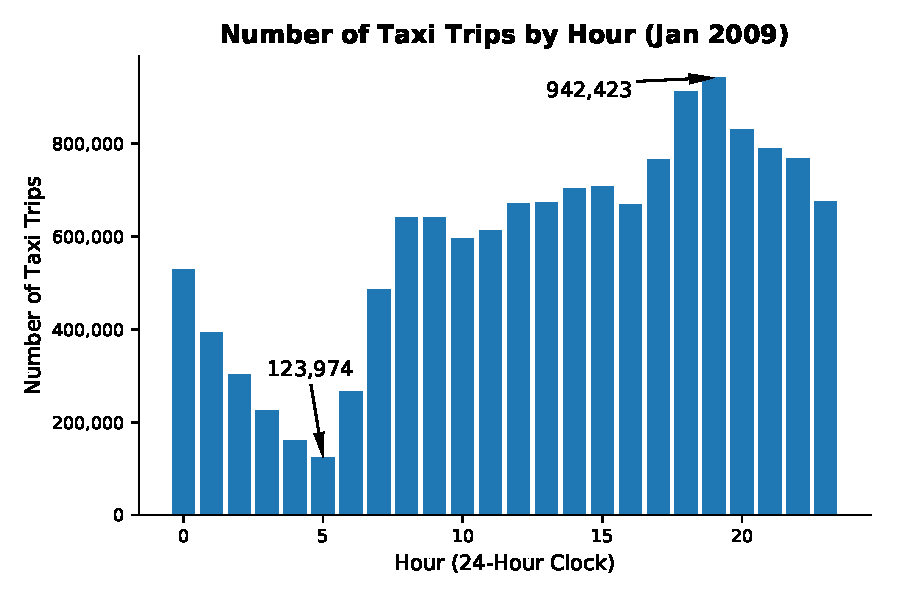
\includegraphics[width=0.5\textwidth]{figs/ridesbyhour.pdf}
\caption{Taxi trips by time of day}
\label{fig:ridesbyhour}
\end{figure}

When we aggregate by hour of day (Figure \ref{fig:ridesbyhour}), we see some variance with anywhere between
a hundred thousand and a million trips per interval. This is reassuring for
future bucketing of the data. 


\begin{figure}[h]
\centering
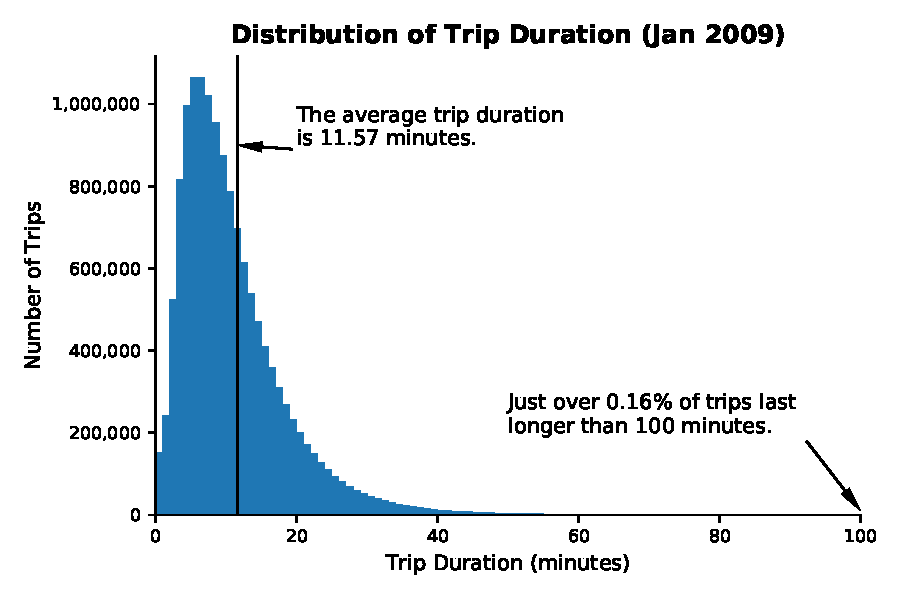
\includegraphics[width=0.5\textwidth]{figs/tripdurations.pdf}
\caption{Taxi trips by duration}
\label{fig:tripdurations}
\end{figure}

While we are not lacking in data volume, two important challenges do appear when
working with this dataset. The first is that the data set is not completely clean.
Case in point, while most trip durations (Figure \ref{fig:tripdurations}) are
reasonable for a taxi trip, just over 1\% of trips have a drop-off time that is
before the pick-up time, making for a trip with negative duration. Furthermore,
the longest trip has duration of just over 42 days. It is difficult to
accurately assess
the veracity of the pickup and dropoff coordinates, but we observe
that some trips
have geographic coordinates that place the start or end of the trip in the
ocean.

Additionally, whereas we would like to infer road conditions along the route of
a taxi trip, we can only observe the start and end-points. The fact that the
route taken is unobservable is primarily responsible for our inference
challenges.


\section{Related Work}
\label{sec:related}

% Example Structure:
% \begin{itemize}
% \item What 3-5 papers have been published in this space?
% \item How do these  differ from your approach?
% \item What data or methodologies do each of these works use?
% \item How do you plan to compare to these methods?
% \end{itemize}

Travel time prediction has historically been a topic of research interest. On a problem of freeway travel time prediction, \citet*{van2002freeway} proposed a Recurrent Neural Network (RNN) approach in order to address the temporal aspect of traffic prediction; \citet*{wu2004travel} adopted the Supportive Vector Regression (SVR) method applied to time-series analysis and reduced prediction errors in cases where previous methods generate especially large errors. We notice that earlier papers share the common feature of using freeway data for training and prediction, which probably arises from the limited availability of GPS data sources. Nevertheless, we realize that even for freeways, which in general have less congestion than city roads, there is evidence that there exists a high level of non-linearity in the data, which contributes to the good performance of models such as RNN and SVR.

With the ubiquity of taxi GPS data, recent work focused on estimating the traffic conditions in cities using sparse probe data---a time series of closely spaced GPS location data for each trip---and used travel time predictions as the metric as the performance of the model. \citet*{hunter2009path} used a Bayesian framework and used an Expectation-Maximization algorithm that simultaneously learns the likely paths taken by probe vehicles as well as the travel time distributions through the network; \citet*{herring2010estimating} used a Coupled Hidden Markov Model (CHMM) and determines the most likely path by allocating the travel time between two consecutive location observations to roads in the M-step of the EM algorithm.

Compared to previous work in the literature, we have much more missing information. Instead of sparse probe data, we are only working with start and end locations, which presents much more challenges in actual path inference and parameter optimization. \citet*{zhan2013urban} provided some very helpful insights since it used the same TLC dataset of taxi ride. They constructed a faithful representation of the Manhattan streets network, but limited the discussion to a much smaller district in Manhattan to reduce computational complexity. Moreover, \citet*{zhan2013urban} also used a softmax regression model for path selection (as detailed in Section~\ref{sec:softmax}), but only restricting the choice set to the 20 shortest paths. Our contribution relative to \citet*{zhan2013urban} is twofold: First, our work scales to the entirety of Manhattan by sacrificing the minute realism of their model and discretizing the Manhattan road network as a simply a grid; second, we employs a novel sampling-based approach to estimate the softmax regression model, so as to drastically expand the choice set of drivers in our model.

\section{Model}
\label{sec:model}

We represent a city's road network with a connected graph $G = (V,E)$. Assume that each vertex $i \in V$ is associated with a weight $w_i$, representing the cost of traversing vertex $i$. A trip is represented by a path in $G$, and the distribution of the trip's duration depends on the weights $w_i$ of vertices included in the path. Note that the choice of the path can in general depend on the collection of weights $\bm W$. In full generality, the model is represented by Figure~\ref{fig:dgm}, where trips in the data are indexed by $(k)$, $T\uppr{k}$ is the observed trip duration, and $Z\uppr{k}$ is the path taken by trip $k$, a latent variable. Our primary interest is to perform inference on $\bm W$, so as to learn the levels of congestion associated with each vertex in $G$. 

\begin{figure}[h]
  \centering
  \caption{Representation of model as a directed graph}
  \label{fig:dgm}
  \vspace{1em}
  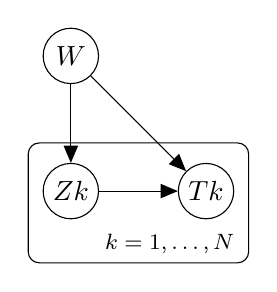
\begin{tikzpicture}
    \node[latent] (W) {$\bm W$};
    \node[latent, below=of W] (Z) {$Z\uppr{k}$};
    \node[latent, right=of Z] (T) {$T\uppr{k}$};
    \edge{W} {Z};
    \edge{W, Z} {T};
    \plate[inner sep=0.5em, yshift=0.2em] {ZT} {(Z) (T)} {$k=1,\ldots,N$} ;
  \end{tikzpicture}
\end{figure}

\subsection{Parameterization}

In principle, in our application to the New York City taxi data, we may take $G$ to be a graph representing the exact road network in New York City, where each vertex is a \emph{road segment} and the directed edge $(i,j) \in E$ if one can drive directly onto road segment $j$ from road segment $i$; such a parameterization allows $w_i$ to be directly interpretable as a measure of congestion on road segment $i$. However, such a detailed construction presents serious computational challenges when training on a large dataset, since solving path-finding problems and computing minimal paths are nontrivially expensive.\footnote{Manhattan has on the order of $10^4$ road segments, and the dataset contains the order of $10^7$ trips for January 2009 alone.} 

To avoid these challenges, we parameterize $G$ as an undirected rectangular grid. Despite not being able to pinpoint weights $w_i$ to congestion of specific road segments, we are nonetheless able to interpret the weights $w_i$ as representative of congestion on a small patch of land. We may now represent a path $Z\uppr{k}$ as a set of indices $i$ of grid points traversed by the path. In full generality, there are an infinite number of paths connecting any two points $i,j$ on the grid, but the vast majority of these paths are not sensible. Thus we restrict the set of possible paths for trip $k$ to a \emph{set of reasonable paths} $\bm Z\uppr{k}$, where each path in $\bm Z\uppr{k}$ travels strictly in the direction of the destination. For instance, if the destination of $j$ is to the northeast of the starting location $i$, then the set of reasonable paths $\bm Z$ are the set of paths that only involve northward or eastward movements (e.g.~Figure~\ref{fig:reasonable} shows a reasonable path from $(0,0)$ to $(2,1)$). Such a parameterization is more general than many in the literature; \citet{zhan2013urban}, for instance, uses the $K$-shortest path algorithm and considers the shortest 20 paths as a set of reasonable paths.

\begin{figure}[h]
\centering
\caption{An example of a reasonable path}
\vspace{1em}

\label{fig:reasonable}
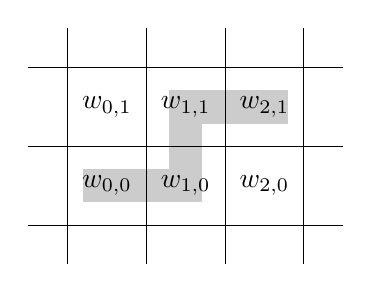
\begin{tikzpicture}
\draw (-0.5,0) -- (3.5,0);
\draw (-0.5,1) -- (3.5,1);
\draw (-0.5,2) -- (3.5,2);

\draw (0,-0.5) -- (0,2.5);
\draw (1,-0.5) -- (1,2.5);
\draw (2,-0.5) -- (2,2.5);
\draw (3,-0.5) -- (3,2.5);

\foreach \y in {0,1}
{
  \foreach \x in {0,...,2}
  {
    \node at (\x+.5,\y+.5) {$w_{\x,\y}$};
  }
}

\draw[line width = 12pt, opacity=.2] (0.2,.5) -- (1.5,.5) -- (1.5,1.5) -- (2.8,1.5);
\end{tikzpicture}
\end{figure} 

We parameterize the conditional distribution of $T\uppr{k}$ as Normal, in the following reformulation of the directed graphical model: \begin{align*}
\bm W &\sim p(\bm W) \\
Z\uppr{k} &\sim p(Z\uppr{k} | \bm W) \\
T\uppr{k} | \bm W, Z\uppr{k} &\sim \Norm\pr{\sum_{i\in Z\uppr{k}} w_i, \sigma^2},
\end{align*}
where $p(Z\uppr{k} | \bm W)$ is a distribution over $\bm Z^{\uppr{k}}$. We consider two different ways to parameterize $p(Z\uppr{k} | \bm W)$: softmax regression and uniform. In the \emph{softmax regression} model, a type of generalized linear model for discrete choice problems \cite{mcfadden1973conditional}, we parameterize the route choice such that \[
p(Z\uppr{k}|\bm W) \propto \exp\pr{-\sum_{i\in Z\uppr{k}}w_i},
\]
in order to encode the fact that drivers avoid routes that take a long period of time. In the \emph{uniform} model, we simply assume that route choice is independent and uniform on the set of reasonable paths: \[
p(Z\uppr{k}|\bm W) \propto 1.
\]
The uniform model trades off realism in modeling for improvement in computation and training, as we see in Section~\ref{sec:inference}.

In our application to the Manhattan dataset, we perform MLE inference, or, equivalently, MAP inference with $p(\bm W) \propto 1$. In principle, it is not difficult to parameterize the prior of $\bm W$ as an undirected graphical model, since we need only to supply edge and unary potentials. For instance, to impose a correlated prior on $\bm W$, as suggested by \citet*{hunter2009path}, we simply penalize large differences in neighboring weights in the edge potential, effectively assuming a prior model that is similar to a continuous version of the Ising model. 



% {
% \color{gray}
% Example Structure:
% 
% \begin{itemize}
% \item What is the formal definition of your problem?
% \item What is the precise mathematical model you are using to represent it? In almost all cases this will use the probabilistic language from class, e.g.
%   \begin{equation}
%   z \sim {\cal N}(0, \sigma^2)\label{eq:1}
% \end{equation}
% But it may also be a neural network, or a non-probabilistic loss,
% \[ h_t \gets \mathrm{RNN}(x_{t}, h_{t-1} )\]
% 
% % Commented out dangling reference --FR
% This is also a good place to reference a diagram such as %Figure~\ref{fig:diagram}.
% 
% \item What are the parameters or latent variables of this model that you plan on estimating or inferring? Be explicit. How many are there? Which are you assuming are given? How do these relate to the original problem description?
% \end{itemize}
% }





% \begin{figure}
%   \centering
%   \missingfigure[figheight=8cm]{}
%   \caption{\label{fig:diagram} This is a good place to include a diagram showing how your model works. Examples include a graphical model or a neural network block diagram.}
% \end{figure}


\section{Inference}
\label{sec:inference}
We perform maximum likelihood inference, maximizing \[
\max_{\bm W} \log p(\{T\uppr{k}\}_{k=1}^N|\bm W) = \max_{\bm W} \sum_{k=1}^N \log p(T\uppr{k} | \bm W).
\]
The log-likelihood is 
\begin{align*}
&\log p (T\uppr{k} | \bm W) \\
=& \log\pr{\sum_{Z\uppr{k} \in \bm Z\uppr{k}} p(T\uppr{k}|Z\uppr{k},\bm W)p(Z\uppr{k}|\bm W)} \\
=& \log\pr{\E_{Z\uppr{k}}\bk{p(T\uppr{k}|Z\uppr{k},\bm W)}}.
\end{align*}
The expectation is a sum of the size $|\bm Z\uppr{k}|,$ which, for an $m\times n$ trip\footnote{By an $m\times n$ trip, we mean a trip with east-west distance $n$ and north-south distance $m$}, is of $\binom{m+n}{n} \approx \frac{(n+m)^n}{n^n}e^n$ terms. Computing this expectation is the main inference challenge of our project.

\subsection{Uniform Model}

By assuming the uniform model $p(Z|\bm W) \propto 1$, we gain the ability to work with an expectation over $\bm W$ instead of an expectation over $\bm Z$, since the probability that a particular weight is included in a path is readily computable from elementary combinatorics. We maximize an approximate lower bound of the log-likelihood by applications of Jensen's inequality: \begin{align*}
\ell(\bm W) &= \log\pr{\E_{Z\uppr{k}}\bk{p(T\uppr{k}|Z\uppr{k},\bm W)}} \\
&= \log\pr{
\E_{Z\uppr{k}}\bk{
\frac{1}{\sigma\sqrt{2\pi}} e^{
-\frac{1}{2\sigma^2}(T\uppr{k} - \sum w_i)^2
}
}
} 
% p(T\uppr{k}|Z\uppr{k},\bm W)}}
\end{align*}
Note that the Normal density is concave for $|T\uppr{k} - \sum w_i| < \sigma$ and convex otherwise. Applying Jensen's inequality locally, we obtain that \[
B(\bm W) = \frac{1}{2\sigma^2}\pr{T\uppr{k} - \sum_i w_i \pi_i}^2,
\]
where $\pi_i$ is the marginal probability of node $i$ being included in a uniform route,\footnote{$\pi_i$ can be computed analytically. Suppose the source and destination of the trip are $(n,m)$ apart and vertex $i$ is $(a,b)$ away from the source. Then, by elementary combinatorics, \[\pi_i = \frac{\binom{a+b}{a}\binom{n+m-a-b}{n-a}}{\binom{n+m}{n}}\]} is a local lower bound for the negative log-likelihood for trips that we predict poorly and is a local upper bound for trips that we predict well, up to a constant. Thus $B(\bm W)$ is a good approximation of the objective function that is easily computable, involving only $mn$ as opposed to $\binom{m+n}{n}$ terms.


% &\ge -\frac{1}{2\sigma^2}\pr{T\uppr{k} - \E\bk{\sum_{i\in Z\uppr{k}} w_i}}^2 + \text{const.} \tag{$*$} \\
% &= -\frac{1}{2\sigma^2}\pr{T\uppr{k} - \sum_{i} w_i\pi_i}^2 + \text{const.},
% \end{align*}
% where $\pi_i$ is the marginal probability of node $i$ being included in a uniform route.\footnote{$\pi_i$ can be computed analytically. Suppose the source and destination of the trip are $(n,m)$ apart and vertex $i$ is $(a,b)$ away from the source. Then, by elementary combinatorics, \[\pi_i = \frac{\binom{a+b}{a}\binom{n+m-a-b}{n-a}}{\binom{n+m}{n}}\]} Note that $(*)$ is only a lower bound if $T\uppr{k} - \sum w_i$ is small compared to $\sigma^2$, since for small values of $T\uppr{k} - \sum w_i$ relative to $\sigma$, the Normal density is concave, and the inequality follows by Jensen's inequality. We indeed make this assumption. By assuming a structure of $Z|\bm W$, we gain a great deal of convenience in computation, effectively reducing a sum of $\binom{n+m}{n}$ terms to a sum of merely $nm$ terms. 
 
 
\subsection{Softmax Regression Model}
\label{sec:softmax}
We now consider a more realistic but more complex model, where we parameterize $Z|\bm W$ as a GLM, namely as a softmax regression where $p(Z|\bm W) \propto \exp\pr{-\sum_{i\in Z}w_i}$, encoding drivers' preferences for shorter trips. The log-likelihood in this model is \begin{align*}
& \ell(\bm W) \\
=& \log\pr{\E_{Z\uppr{k}}\bk{\frac{1}{\sqrt{2\pi}\sigma} e^{-\frac{1}{2\sigma^2}(T\uppr{k} - \sum_i w_i)^2}}}\\
=& \log\pr{\sum_{Z\uppr{k}\in \bm Z\uppr{k}} \frac{1}{\sqrt{2\pi}\sigma} e^{-\frac{1}{2\sigma^2}(T\uppr{k} - \sum_i w_i)^2} p(Z\uppr{k}|\bm W)}
\end{align*}

Before we discuss our inference strategy, we first discuss a few difficulties of the model. At first glance, the latent variable structure seems lend well to the Expectation-Maximization algorithm \cite{dempster1977maximum}. However, the EM algorithm requires computing the term \[
Q(\bm W|\bm W\uppr{t}) = \E\pr{\log(T\uppr{k}, Z\uppr{k} | \bm W) | T\uppr{k}, \bm W\uppr{t}},
\]
and computing the expectation requires the conditional distribution $p(Z | T, \bm W) = \frac{p(T|Z,\bm W)p(Z|\bm W)}{p(T|\bm W)}$, where the denominator is intractable to compute. We might also consider techniques in variational inference \cite{blei2017variational}. However, the latent variable $Z\uppr{k}$ is a random set of indices with the property that the indices form a path on the grid, and thus cannot be reasonably decomposed into independent components, ruling out the mean-field algorithm. Another promising option is stochastic gradient variational Bayes (SGVB) and variational autoencoders \cite{kingma2013auto}, which is designed for large datasets for which the EM algorithm fails. However, SGVB requires a reparameterization of the latent variable drawn from an approximate distribution, in order for the gradients to be properly computed. In SGVB, one independently draws some $\epsilon$ from a distribution and obtains $z$ via $z = g(\epsilon)$ for some continuous function $g$.\footnote{Here we are using the notation in \cite{kingma2013auto}.} This is difficult to do in our context, since $Z$ is not continuous nor scalar-valued. Thus it is difficult to find an $\epsilon$ and a continuous transformation to approximate samples from the distribution of $Z$.  

Our inference strategy is based on a sampling-based approximating to the expectation over $\bm Z$. The key trick we use is that 
\begin{equation}
\label{eq:trick}
  \E_{Z}\bk{f(Z\uppr{k})} = |\bm Z\uppr{k}| \E_{\tilde Z}\bk{f(\tilde Z\uppr{k})p_Z(\tilde Z\uppr{k}|\bm W)},
\end{equation}
where $\tilde Z$ is drawn uniformly from $\bm Z$. This is the same technique as in importance sampling, except here the objective is to derive computationally tractable approximations, rather than maximizing the efficiency of the approximations. Exchanging $\log$ and expectation operator and applying \eqref{eq:trick} yields the following upper bound for negative log-likelihood, up to a constant,
\begin{align}
&\frac{1}{2L\sigma^2}\sum_{j=1}^L \bk{T\uppr{k} + \sum_{i\in \tilde Z\uppr{k}_j}w_i}^2 + \frac{1}{L}\sum_{i=1}^L\sum_{i\in\tilde Z_{j}\uppr{k}}w_i 
\label{eq:softmax_objective}
\\&\qquad + \underset{i=1,\ldots,L}{\text{logsumexp}}\pr{-\sum_{\tilde Z_i} w_i} \nonumber,
\end{align}
where we sample uniformly and independently $\{\tilde Z_j\uppr{k}\}_{j=1}^L$. The pseudocode of the implementation is detailed in Algorithm~\ref{alg:main_alg}.

\begin{algorithm}
  \begin{algorithmic}
    \STATE{\COMMENT{Optimizing using \texttt{torch.optim.Adam}}}
    
    \FOR{trip $k$ in $1,\ldots,N$} \STATE {
    Sample $L$ random paths uniformly.
    
    Compute the objective function as in~\eqref{eq:softmax_objective} for observation $k$.
    
    Compute the gradients of the objective function with respect to $\bm W$.
    
    Update $\bm W$.
    } \ENDFOR
  \end{algorithmic}
  \caption{Training algorithm for softmax path selection}
  \label{alg:main_alg}
\end{algorithm}


\subsection{Prediction}
\label{sub:predict}
We conclude this section by briefly discussing prediction in our models. In the uniform model, prediction is straightforward. We calculate the expected time $\hat T = \sum_i w_i \pi_i$, where $\pi_i$ is the marginal probability that node $i$ is included in a uniformly randomly chosen path. Computing prediction is slightly more subtle in the softmax regression model. In the softmax regression model, we sample $L_{\text{pred}}$ uniformly chosen paths and take the weighted average of the sums of $w_i$ in each path, where the weights are proportional to $\exp(-\sum_{i \in Z} w_i)$ for path $Z$. 

% {\color{gray}
% \begin{itemize}
% \item How do you plan on training your parameters / inferring the
%   states of your latent variables (MLE / MAP / Backprop / VI / EM / BP / ...)

% \item What are the assumptions implicit in this technique? Is it an approximation or exact? If it is an approximation what bound does it optimize?

% \item What is the explicit method / algorithm that you derive for learning these parameters?
% \end{itemize}

% }




\section{Methods}
\label{sec:methods}

% {
% \color{gray}
% \begin{itemize}
% \item What are the exact details of the dataset that you used? (Number of data points / standard or non-standard / synthetic or real / exact form of the data)
% 
% \item What are the exact details of the features you computed?
% 
% \item How did you train or run inference? (Optimization method / hyperparameter settings / amount of time ran / what did you implement versus borrow / how were baselines computed).
% 
% \item What are the exact details of the metric used?
% \end{itemize}
% }

\subsection{Data Processing}

For our dataset, we started with the TLC dataset of all NYC taxi trips taken in
January 2009. From the raw data, we added several computed columns.
We one-hot-encoded columns for hour of day (24 columns) as well as for
day of the week (7 columns). We also explicitly computed the duration of the trip  in seconds as the dependent variable to predict.

In addition to adding columns, we filtered the original dataset. We only consider trips
whose start- and end-locations that falls inside a rectangle that bounds Manhattan. We also removed trips with duration less than two minutes or more than two hours.

We performed a principal component analysis on all de-meaned and
standardized geographic coordinates (both start
and end locations) from the filtered data. We thus transform the coordinates into the first and second principal components. This allowed us to compute the rotational matrix so that Manhattan lies approximately orthogonal to the $x$-axis. For the discrete
grid models, these coordinates were further discretized into a $20 \times 70$
grid. Each node in the grid approximately corresponds to a $400\text{ft} \times 400\text{ft}$ area. We chose the grid size as a compromise between computational tractability and model expressiveness.

We saved the dataset as a whole, and we also partitioned into $(\text{day of week},
\text{hour})$ groups, using the one-hot encoded vectors. Some models were
trained on the entire dataset (e.g.\ Neural Network), and some were trained
individually on the partioned datasets (e.g.\ Structural Models).

\subsection{Baselines}

We calculated three baselines. The first was a linear regression predicting
trip duration from trip distance (calculated using the Pythagorean Theorem and
the start and end coordinates), and trained on a partitioned data set. 

The second was a neural network trained on the
entire dataset taking as input the start and end coordinates as well as the day
of week and hour one-hot encoded vectors. The neural network had one hidden
layer with 50 neurons and a $\tanh$ activation function.

The third baseline was constructed by querying the Google Maps Distance Matrix
API.\footnote{\url{https://developers.google.com/maps/documentation/distance-matrix/}}
While there was no need to train this baseline, there was a rate limit
constraint on how many test data points it could be tested on. We assess its
performance on 2,500 data points in a representative partioned test dataset.

\subsection{Training}

Training implementations varied from model to model. In training the neural
network baseline, SGD was used with a learning rate of $10^{-7}$ run for 12
epochs on the full data set. This took between 30 minutes and an hour. The
uniform paths structural model was similarly trained with SGD, with a learning
rate of $10^{-4}$. 

The uniform model was only trained on a subset of the
dataset corresponding to all trips on a given day of the week and on a given
hour. Convergence appeared after roughly two epochs, and the model was run for 5
epochs taking just under ten minutes.

The softmax regression model was trained
using the Adam optimizer \cite{kingma2014adam} with learning rate $10^{-2}$ for 10 epochs,
taking approximately an hour. Additionally, the softmax regression model take hyperparameters $L$ (sample size in each stochastic draw) and $\sigma^2$ (variance of trip time). We chose $L = 20$ and $\sigma^2 = 100$. These values are again chosen to strike a bargain between realism and computation feasibility. The model appears to converge by the second epoch. 

\section{Results}
\label{sec:results}


% {\color{gray}\begin{itemize}
% \item What were the results comparing previous work / baseline systems / your systems on the main task?
% \item What were the secondary results comparing the variants of your system?
% \item This section should be fact based and relatively dry. What happened, what was significant?
% \end{itemize}
% }


\begin{figure}[h]
\centering
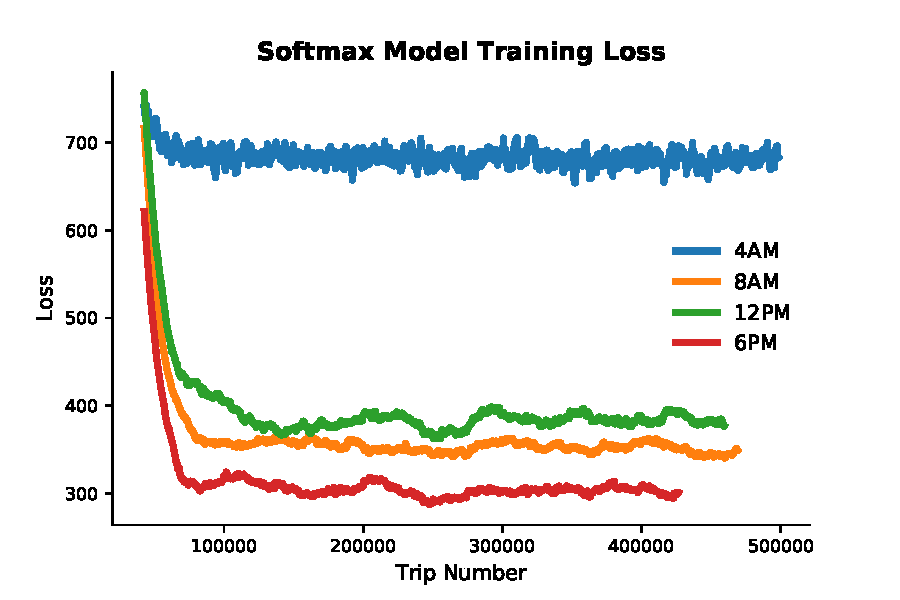
\includegraphics[width=0.5\textwidth]{figs/softmaxloss}
\caption{Softmax model training loss, rolling average}
\label{fig:softmaxloss}
\end{figure}

We train our model and test the model on an out-of-sample test-set using the methods discussed in Section~\ref{sub:predict}. As a simple check of the training process, we plot in Figure~\ref{fig:softmaxloss} the loss obtained when fitting the softmax regression model. We see that the model converges relatively fast.\footnote{The full fitting takes approximately 30 minutes per dataset (2.9 GHz Intel Core i5, 8GB RAM), but the model appears to converge in only 20\% of that time.} The convergence plot for the uniform model is extremely similar and thus omitted. Table~\ref{tab:mainres} contains the main prediction results of our model relative to some benchmark predictions
such as the Google Maps Distance Matrix API, neural network, and linear regression. We note that, in terms of predictive metrics, our models were able to outperform Google Maps and linear regression, but were not able to outperform the neural network, even though the difference is not very large. Despite the disappointing outcome, the advantage of our framework is that the parameters have structural interpretations, whereas the neural network is a black box. 

\begin{table*}[h!]
\centering
\begin{threeparttable}
\begin{tabular}{lrrrrr}
\toprule
& \multicolumn{3}{c}{Baseline} & \multicolumn{2}{c}{Model} \\\cmidrule(r){2-4} \cmidrule(l){5-6} 
{} & Google Maps & Neural Network\tnote{2} & Linear Regression\tnote{3} & Uniform Model & Softmax Model \\
\midrule
$\sd(T)$ & 7.40 & 6.85& 6.13&  6.22 & 6.22 \\ [1em]
$\hat \E[\epsilon]\tnote{1}$ & -0.83 &-0.07 & -0.05&  0.61 & 0.99 \\
$\sd(\epsilon)$ & 4.98 & 3.88& 5.01&  4.28 & 4.28 \\[1em]
$\hat \E[|\epsilon|]$ & 3.42 & 2.44& 3.60&  2.82 & 2.86 \\
$\text{Median}(|\epsilon|)$ & 2.55 & 1.67& 2.93 &  1.92 & 1.92 \\
$\text{Percentile}(|\epsilon|, 99)$ & 16.54 &12.79 & 16.62&  14.72 & 15.24 \\ [1em]
Test-set\tnote{4}  \, $R^2$ & 0.54 & 0.68& 0.33 & 0.53 & 0.53 \\
\bottomrule
\end{tabular}
\caption{Prediction results on test set}
\label{tab:mainres}
\begin{tablenotes}
% \item[\textbf{Notes:}]
\item[1] Here $\epsilon = (\text{Actual trip duration}) - (\text{Predicted duration})$ in minutes. $\hat \E$ denotes the sample mean. 
\item[2] We restrict the test-set to 8:00--9:00 AM on Tuesdays in January 2009 for all models \emph{except} the neural network, for which we use an out-of-sample test set on the \emph{entire} range of trip times, since the neural network encodes time-of-day and day-of-week data. 
\item[3]In linear regression, we simply regress $T$ on straight-line distance between the source and the destination.  
\item[4] Test-set $R^2$ is calculated as \smash{$1-\frac{\var(\epsilon)}{\var(T)}$} on the underlying dataset being tested on. Note that the test-set $R^2$ is an out-of-sample $R^2$. 
\end{tablenotes}
\end{threeparttable}
\end{table*}


\section{Discussion}
\label{sec:discuss}

% table
%  


Table~\ref{tab:mainres} is encouraging. Our models successfully leverage the power of geography and picks up more signal in the data than distance of the trip alone, as demonstrated by the significantly improved performance over linear regression. Perhaps more strikingly, our model slightly outperforms the predictions generated by Google Maps, which means that the predictive accuracy of the model is on par with the standard of a widely used consumer product. Even though we were not able to outperform the neural network, we reiterate that the main advantage of our approach is to have interpretable parameters, which are visualized in Figure~\ref{fig:unifmap}. We turn to the figure in the next section.
% \begin{itemize}
% \item What conclusions can you draw from the results section?
% \item Is there further analysis you can do into the results of the system? Here is a good place to include visualizations, graphs, qualitative analysis of your results.
% \item  What questions remain open? What did you think might work, but did not?
% \end{itemize}

\begin{figure}[h!]
\centering
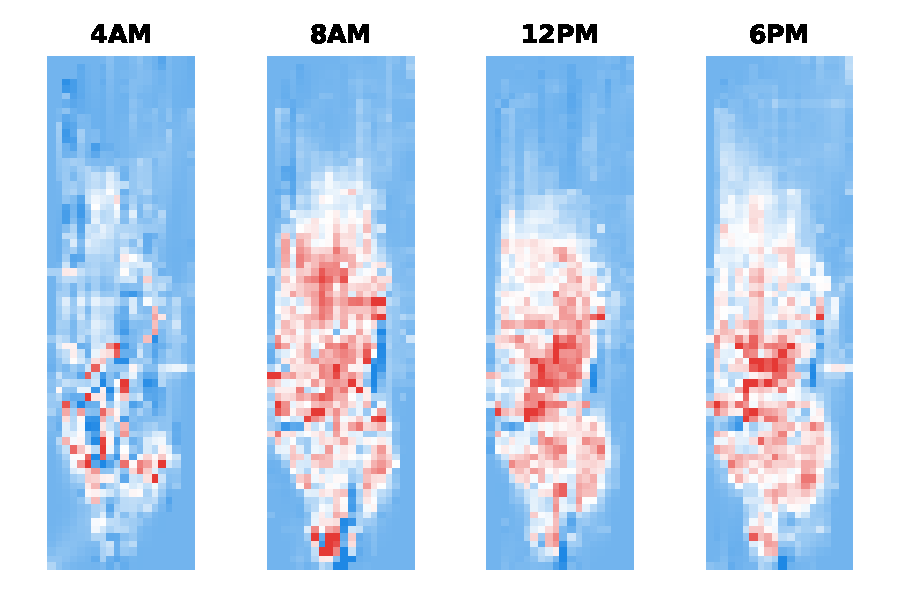
\includegraphics[width=0.5\textwidth]{figs/unifmaps.pdf}
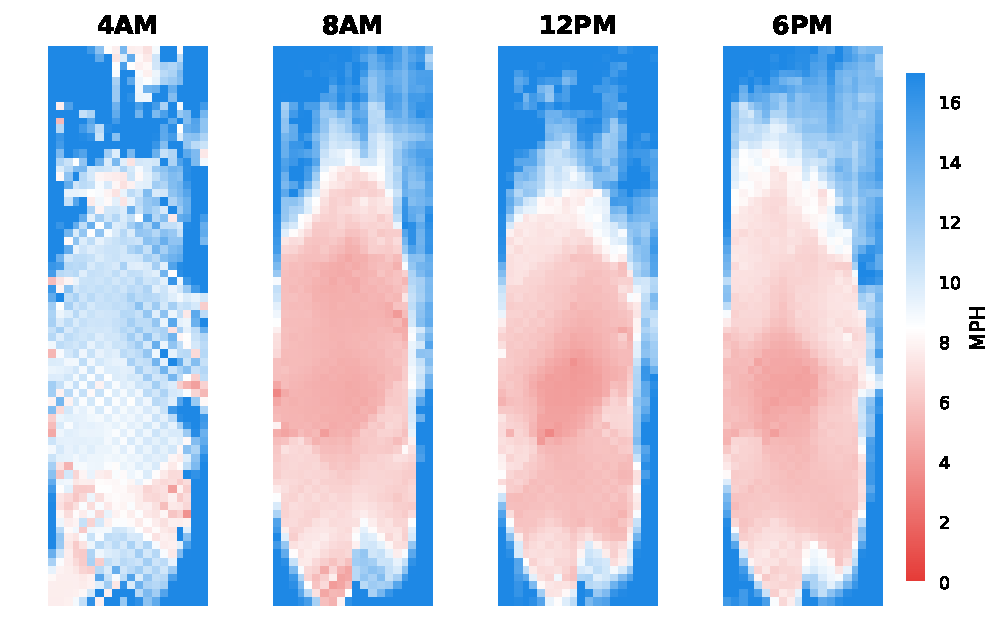
\includegraphics[width=0.5\textwidth]{figs/softmaxmaps.pdf}
\caption{Learned weights, various times Tuesday. Top row: uniform model.
Bottom row: softmax model.}
\label{fig:unifmap}
\end{figure}

\subsection{Comparing Models}

Figure~\ref{fig:unifmap} shows that the parameter values for the uniform and softmax regression models behave similarly, with similar areas of high and low congestion. The patterns seem to largely agree with conventional wisdom, both in spatial and temporal dimensions. We identify that 4:00 AM is indeed less congested than rush hour, that Midtown Manhattan seems to be particularly congested during the day, and that the congested areas have an average speed of 4--6 miles per hour. The visualization also confirms some less-than-well-known features; the areas that demonstrate congestion at 4:00 AM largely confirms with anecdotal evidence.\footnote{According to \textit{Business Insider} (\url{http://read.bi/164vSK1}), East Village and surrounding areas rank highly for nightlife. %#GETLIT
} As the models seem to produce largely similar output, we conclude that they are fairly robust.

However, the two models do have significant differences. The softmax regression model appears to have smoother parameter values than the uniform model. This is consistent with the softmax model ascribing higher probability to faster paths, and so we expect the parameter updates to spread out spatially.

It is difficult to select the model to use based on predictive metrics alone, as the models perform strikingly similarly. However, from a practical standpoint, the uniform model is significantly easier to implement and faster to train than the softmax regression model, even though the latter embraces more structural realism. 

% For instance, both models identify an interesting feature of the traffic patterns in Manhattan, where it is less congested east of Broadway in lower Manhattan than west of Broadway---we speculate that 



\subsection{Remaining Puzzles}

While many of our results make sense in the context of the models that produce
them, some puzzles---both qualitative and quantitative---remain. For instance,
visual inspection of the grid of weights that the softmax model converges to
(see bottom row of Figure \ref{fig:unifmap}) reveals a pattern that resembles a
checkerboard. This behavior is most visible in the 4:00 AM weights, but also
appears in certain areas of the other grids. We suspect this has to do with the
superimposition of paths that we train on, but the result largely remains an
unexpected surprise.

Furthermore, we are also intrigued by the bias our models introduce: both the
uniform and softmax structural models on average underestimate trip duration
(see Table \ref{tab:mainres}). Since we optimize an approximate bound, it
is believable that this procedure introduced bias. Nevertheless, we are
missing a good intuition as to why we systematically underestimate and whether
this is a feature or a bug.

\subsection{Future Work}

In thinking of ways to develop our work further, a couple of directions come to
mind. Foremost among them is taking a closer look at which of the softmax and
uniform models best captures reality. They perform very similarly on our
test data, but their weights correspond to structurally different maps of
Manhattan. Future work could help determine which of these depictions best
tracks actual traffic conditions.

In addition, our models currently train from scratch on each partition of the
data. However, it is not hard to imagine that, for example, traffic conditions
at 8:00 AM on Tuesdays can tell you something about conditions at 9:00 AM on
Tuesdays, or 8:00 AM on Wednesdays. Exploring ways to leverage this structure
through transfer learning could significantly speed up the training of our
models.


% checkboard?
% bias?
% unclear how to decide which one is better
% improve the softmax one??
% transfer learning from different times


% \begin{itemize}
% \item What conclusions can you draw from the results section?
% \item Is there further analysis you can do into the results of the system? Here is a good place to include visualizations, graphs, qualitative analysis of your results.
% 
% \end{itemize}

% \begin{figure}
%   \centering
%   \missingfigure{}
%   \missingfigure{}
%   \missingfigure{}
%   \caption{Visualizations of the internals of the system.}
% \end{figure}

\section{Conclusion}
\label{sec:conc}



%% Feature extraction from parameter values 

% \section*{Acknowledgements}

% \textbf{Do not} include acknowledgements in the initial version of
% the paper submitted for blind review.

% If a paper is accepted, the final camera-ready version can (and
% probably should) include acknowledgements. In this case, please
% place such acknowledgements in an unnumbered section at the
% end of the paper. Typically, this will include thanks to reviewers
% who gave useful comments, to colleagues who contributed to the ideas,
% and to funding agencies and corporate sponsors that provided financial
% support.

\bibliography{biblio.bib}
\bibliographystyle{icml2017}

\end{document}
